\documentclass{article}
\usepackage[margin=0.5in]{geometry}
\usepackage{Sweave}
\begin{document}
\Sconcordance{concordance:hw3_saket.tex:hw3_saket.Rnw:%
1 2 1 1 0 7 1 1 2 1 0 1 1 3 0 1 2 1 1 1 2 1 0 1 1 15 0 1 2 3 1 1 2 1 0 %
1 3 2 0 1 5 8 0 1 2 3 1 1 2 1 0 2 1 15 0 1 2 4 1 1 2 1 0 1 1 25 0 1 2 2 %
1 1 2 1 0 1 1 1 3 2 0 1 5 8 0 1 2 4 1 1 2 8 0 1 2 1 1 1 2 16 0 1 2 1 1 %
1 2 16 0 1 2 7 1 1 2 15 0 2 1 1 3 2 0 1 5 8 0 1 2 4 1 1 2 8 0 1 2 1 1 1 %
2 16 0 1 2 4 1 1 2 16 0 1 2 9 1}


%\SweaveOpts{concordance=TRUE}
\title{HW\#3 ||  MDS  Eigen Decomposition using pairwise distances of US cities}
\author{Saket Choudhary}
\maketitle

\begin{Schunk}
\begin{Sinput}
> library(graphics)
> library(ggplot2)
\end{Sinput}
\end{Schunk}

\textbf{Read Data:}
\begin{Schunk}
\begin{Sinput}
> distanceMatrix <- read.csv("distance_matrix.csv", header=T)
> distanceMatrix
\end{Sinput}
\begin{Soutput}
  BOST   NY   DC MIAM CHIC SEAT   SE   LA DENV
1    0  206  429 1504  963 2976 3095 2979 1949
2  206    0  233 1308  802 2815 2934 2786 1771
3  429  233    0 1075  671 2684 2799 2631 1616
4 1504 1308 1075    0 1329 3273 3053 2687 2037
5  963  802  671 1329    0 2013 2142 2054  996
6 2976 2815 2684 3273 2013    0  808 1131 1307
7 3096 2934 2799 3053 2142  808    0  379 1235
8 2979 2786 2631 1687 2054 1131  379    0 1059
9 1949 1771 1616 2037  996 1307 1235 1059    0
\end{Soutput}
\end{Schunk}

\section{MDS}
\begin{figure}

\begin{Schunk}
\begin{Sinput}
> mds <- cmdscale(distanceMatrix)
> mdsPlot  <- qplot(x=mds[,1], 
+                   y=-mds[,2], 
+                   label=colnames(distanceMatrix)) 
> mdsPlot + 
+   geom_point(color='red') + 
+   geom_text(hjust=-.15) + 
+   xlab("X1") + ylab("X2") + 
+   ggtitle("MDS plot using 2 dimensions")
\end{Sinput}
\end{Schunk}
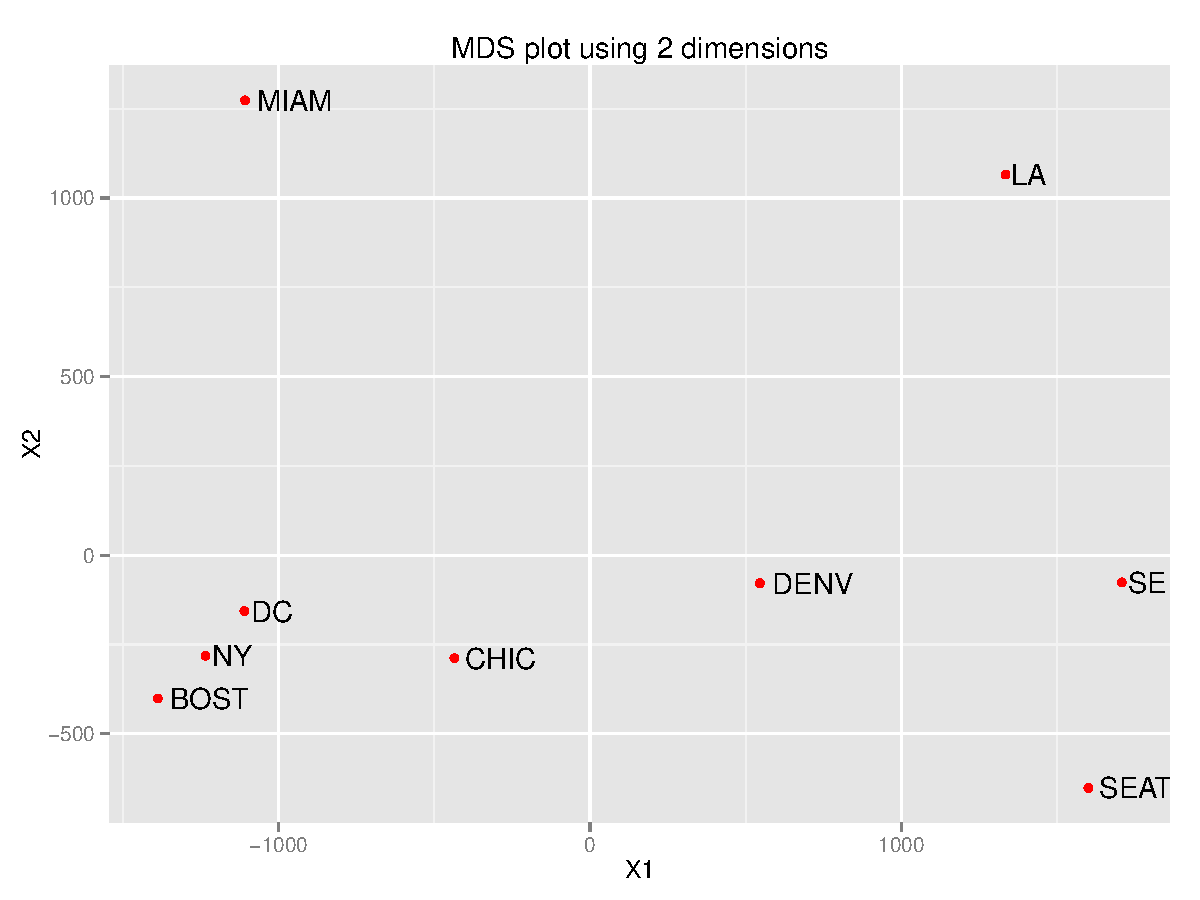
\includegraphics{hw3_saket-003}
\caption{MDS plot(2D)}
\end{figure}

Coordinates of points are given by:
\begin{Schunk}
\begin{Sinput}
> rownames(mds) <- colnames(distanceMatrix)
> colnames(mds) <- c("X1", "X2")
> print(mds)
\end{Sinput}
\begin{Soutput}
             X1          X2
BOST -1388.4759   401.09561
NY   -1235.5455   281.49474
DC   -1110.4073   156.62867
MIAM -1108.0546 -1273.17629
CHIC  -435.5452   288.46936
SEAT  1601.4477   651.49498
SE    1708.7378    76.02141
LA    1335.1428 -1065.44210
DENV   546.1006    78.38664
\end{Soutput}
\end{Schunk}
%\end{figure}

\section{EigenValue Decomoposition}
\subsection{Using similarity matrix}

\begin{Schunk}
\begin{Sinput}
> similarityMatrix <- apply(distanceMatrix, 1, function(x) exp(-x^2/3000.0^2))
> similarityMatrix
\end{Sinput}
\begin{Soutput}
          [,1]      [,2]      [,3]      [,4]      [,5]      [,6]      [,7]
BOST 1.0000000 0.9952960 0.9797587 0.7777617 0.9020900 0.3737889 0.3447196
NY   0.9952960 1.0000000 0.9939860 0.8268797 0.9310269 0.4145882 0.3842415
DC   0.9797587 0.9939860 1.0000000 0.8794991 0.9512040 0.4491365 0.4187467
MIAM 0.7777617 0.8268797 0.8794991 1.0000000 0.8218076 0.3041358 0.3549972
CHIC 0.9020900 0.9310269 0.9512040 0.8218076 1.0000000 0.6374745 0.6006181
SEAT 0.3737889 0.4145882 0.4491365 0.3041358 0.6374745 1.0000000 0.9300281
SE   0.3449568 0.3842415 0.4187467 0.3549972 0.6006181 0.9300281 1.0000000
LA   0.3730477 0.4221385 0.4634165 0.4483331 0.6257725 0.8675093 0.9841666
DENV 0.6556903 0.7057505 0.7481425 0.6306268 0.8956335 0.8271200 0.8441125
          [,8]      [,9]
BOST 0.3730477 0.6556903
NY   0.4221385 0.7057505
DC   0.4634165 0.7481425
MIAM 0.7289000 0.6306268
CHIC 0.6257725 0.8956335
SEAT 0.8675093 0.8271200
SE   0.9841666 0.8441125
LA   1.0000000 0.8828420
DENV 0.8828420 1.0000000
\end{Soutput}
\end{Schunk}

Perform PCA an similarityMatrix: 
\begin{figure}
\begin{Schunk}
\begin{Sinput}
> similarityMatrix.prcomp <- prcomp(similarityMatrix, scale.=T)
> similarityMatrix.PCA <- similarityMatrix.prcomp$x[,1:2]
> similarityMatrix.plot <- qplot(x=similarityMatrix.PCA[,1],
+                           y=similarityMatrix.PCA[,2], 
+                           label=colnames(distanceMatrix))
> similarityMatrix.plot +
+   geom_point(color='red') +
+   geom_text(hjust=-.15) +
+   xlab("PC1") + ylab("PC2")+
+   ggtitle("First 2 principle components of similarity Matrix")
\end{Sinput}
\end{Schunk}
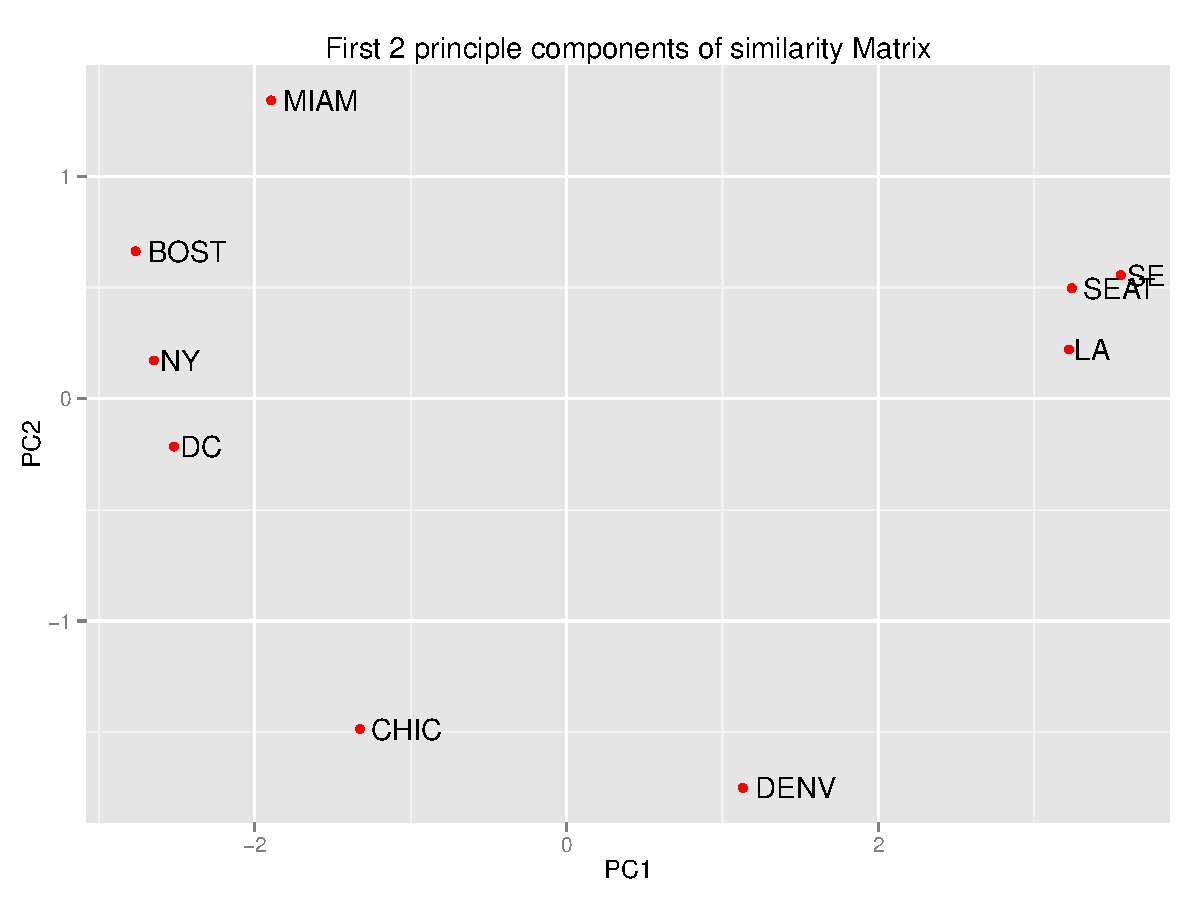
\includegraphics{hw3_saket-006}
\caption{PCA using gaussian kernel(using similarity matrix)}
\end{figure}

\subsubsection{EigenValues}

\begin{Schunk}
\begin{Sinput}
> print(similarityMatrix.prcomp$sdev)
\end{Sinput}
\begin{Soutput}
[1] 2.763748e+00 1.011925e+00 5.609621e-01 1.317532e-01 6.715841e-02
[6] 3.342472e-02 6.485914e-03 1.019860e-03 1.743940e-16
\end{Soutput}
\end{Schunk}

\subsubsection{EigenVectors}
\begin{Schunk}
\begin{Sinput}
> print(similarityMatrix.prcomp$rotation[,1:2])
\end{Sinput}
\begin{Soutput}
             PC1         PC2
 [1,] -0.3552454 -0.15532942
 [2,] -0.3556963 -0.17183709
 [3,] -0.3555762 -0.18252044
 [4,] -0.3372374 -0.03256753
 [5,] -0.3160704 -0.47693301
 [6,]  0.3425956 -0.25501975
 [7,]  0.3540793 -0.19295181
 [8,]  0.3348572 -0.03848530
 [9,]  0.2287874 -0.76207529
\end{Soutput}
\end{Schunk}

\subsubsection{Principle  Components(Scaled and Centered)}
\begin{Schunk}
\begin{Sinput}
> print(similarityMatrix.prcomp$x[,1:2])
\end{Sinput}
\begin{Soutput}
           PC1        PC2
BOST -2.763048  0.6631076
NY   -2.646744  0.1721873
DC   -2.517306 -0.2152715
MIAM -1.894466  1.3418267
CHIC -1.324643 -1.4856597
SEAT  3.240198  0.4969233
SE    3.553513  0.5559057
LA    3.222135  0.2212970
DENV  1.130362 -1.7503165
\end{Soutput}
\end{Schunk}




\subsection{Using distance matrix}

Perform PCA an distanceMatrix: 
\begin{figure}
\begin{Schunk}
\begin{Sinput}
> distanceMatrix
\end{Sinput}
\begin{Soutput}
  BOST   NY   DC MIAM CHIC SEAT   SE   LA DENV
1    0  206  429 1504  963 2976 3095 2979 1949
2  206    0  233 1308  802 2815 2934 2786 1771
3  429  233    0 1075  671 2684 2799 2631 1616
4 1504 1308 1075    0 1329 3273 3053 2687 2037
5  963  802  671 1329    0 2013 2142 2054  996
6 2976 2815 2684 3273 2013    0  808 1131 1307
7 3096 2934 2799 3053 2142  808    0  379 1235
8 2979 2786 2631 1687 2054 1131  379    0 1059
9 1949 1771 1616 2037  996 1307 1235 1059    0
\end{Soutput}
\begin{Sinput}
> distanceMatrix.prcomp <- prcomp(distanceMatrix, scale.=T)
> distanceMatrix.PCA <- distanceMatrix.prcomp$x[,1:2]
> distanceMatrix.plot <- qplot(x=distanceMatrix.PCA[,1],
+                           y=distanceMatrix.PCA[,2], 
+                           label=colnames(distanceMatrix))
> distanceMatrix.plot +
+   geom_point(color='red') +
+   geom_text(hjust=-.15) +
+   xlab("PC1") + ylab("PC2") +
+   ggtitle("First 2 principle components of distanceMatrix")
\end{Sinput}
\end{Schunk}
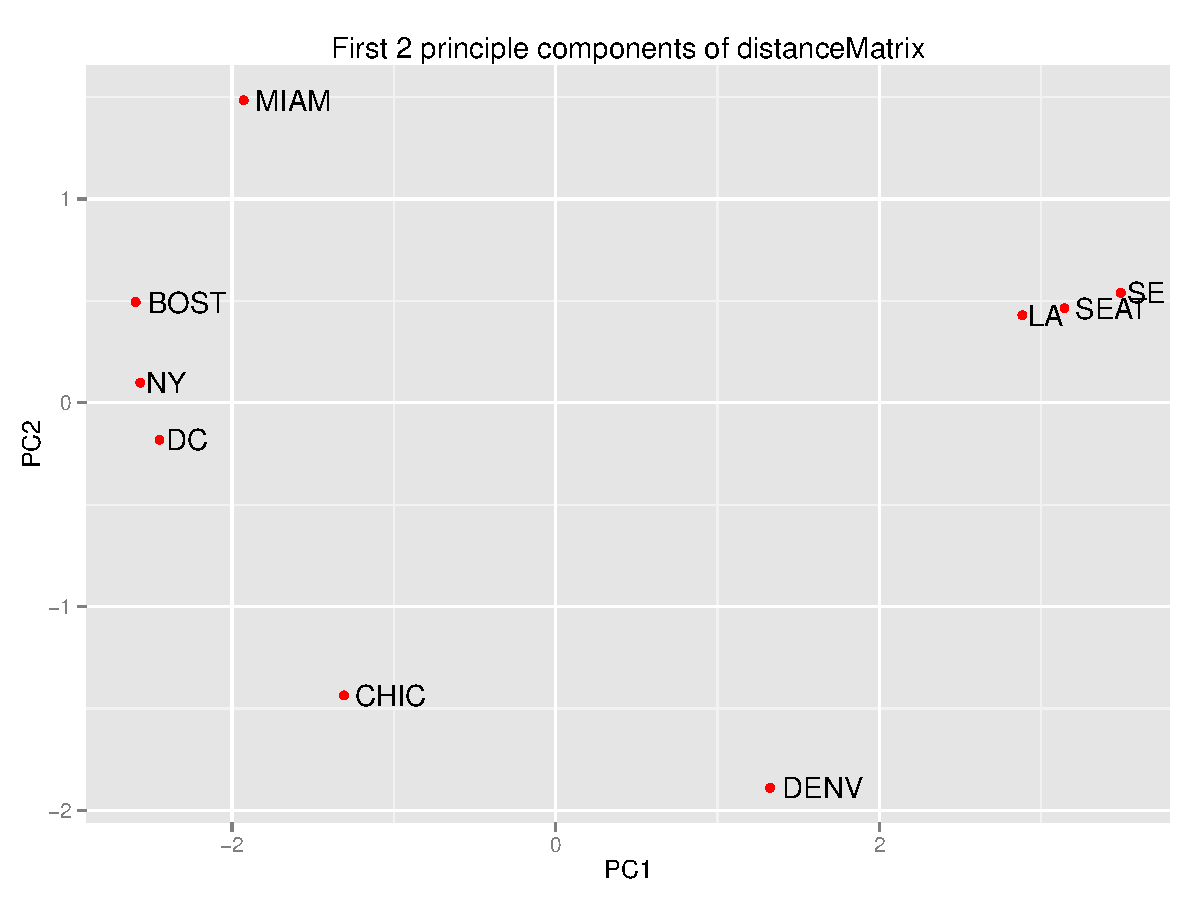
\includegraphics{hw3_saket-010}
\caption{PCA without using gaussian kernel(using distance matrix)}
\end{figure}

\subsubsection{EigenValues}

\begin{Schunk}
\begin{Sinput}
> print(distanceMatrix.prcomp$sdev)
\end{Sinput}
\begin{Soutput}
[1] 2.666684e+00 1.049368e+00 7.363066e-01 3.395746e-01 2.999203e-01
[6] 1.640774e-01 1.070771e-01 4.272792e-02 1.600394e-17
\end{Soutput}
\end{Schunk}

\subsubsection{EigenVectors}
\begin{Schunk}
\begin{Sinput}
> print(distanceMatrix.prcomp$rotation[,1:2])
\end{Sinput}
\begin{Soutput}
            PC1         PC2
BOST  0.3609929  0.13053243
NY    0.3632938  0.14972372
DC    0.3651761  0.17155008
MIAM  0.2962816 -0.13553983
CHIC  0.2957988  0.54249894
SEAT -0.3516124  0.16804789
SE   -0.3676068  0.08877045
LA   -0.3577376  0.10405688
DENV -0.2057333  0.75596984
\end{Soutput}
\end{Schunk}



\subsubsection{Principle  Components(Scaled and Centered)}

\begin{Schunk}
\begin{Sinput}
> print(distanceMatrix.prcomp$x[,1:2])
\end{Sinput}
\begin{Soutput}
            PC1         PC2
 [1,] -2.594727  0.49402847
 [2,] -2.566601  0.09812092
 [3,] -2.448209 -0.18194241
 [4,] -1.927579  1.48379129
 [5,] -1.307785 -1.43547852
 [6,]  3.143991  0.46313051
 [7,]  3.491687  0.53895796
 [8,]  2.883923  0.42915851
 [9,]  1.325301 -1.88976673
\end{Soutput}
\end{Schunk}

\section{Discussion}

As evident from Figure 1 and Figure 2, transforming original data from pairwise distances to pairwise similairties using gaussian kernel does not seem to have effect on the resulting PCA plots. The most probable reasoning is because the data is linearly separable in its original 9 dimensions. With the gaussian kernel trick each row being a 9-D vector is transformed to a infinite-dimensional space(a function for example satisfies all operations that a vector satisfies: addition/multiplication in 'higher' dimensions and with a gaussian kernel with fixed $\sigma^2$ each original vector is sent to a 'higher' dimensional gaussian blob centered at that point. If any two points in original 9-D space were close, their guassian transformation would lead to the resulting vectors having small angle in the 'higher' dimensional space), assuming that higher dimensions would guarantee linear separation. But in this case, linear separation is guaranteed in the original 9-dimensions itself.

\subsection{Equivalence of MDS and PCA?}
MDS and PCA are expected to have same results when eucliden distances are used.
[Cox, Trevor F., and Michael AA Cox. Multidimensional scaling. CRC Press, 2000.]

\end{document}
